\documentclass[12pt,
border=1pt]{standalone}
\usepackage{pgfplots}
\usepackage{amsmath}
\usepackage{amssymb}

\pgfplotsset{compat=newest,
	width=6cm, height=5cm,
	xtick pos=left, ytick pos=left
	%            scaled x ticks=real:1e-6,
}
% Kernel 2 FP64
\begin{document}
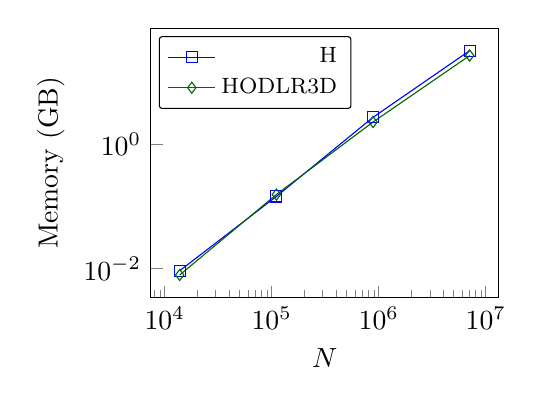
\begin{tikzpicture}
	\begin{axis}[xlabel={$N$},
	ylabel={Memory (GB)},
%		legend pos=south east,
		legend style={
                at={(0.3,0.7)},
               anchor=south,
               legend columns=1,
               cells={anchor=east},
              font=\footnotesize,
               rounded corners=1pt,
               },
		xmode = log,
	    ymode = log,
	   % xmin = 1e3,
	   % xmax = 1e6,
	   % ymin = 1e-10,
	   % ymax = 1e-0,
	   % xtick={1e-10, 1e-8, 1e-6,  1e-4,  1e-2},
	   % ytick={1e-8, 1e-6,  1e-4,  1e-2, 1e-0}
		]
	
		\addplot[
		color=blue,
		mark=square,
		] coordinates {
(13824,0.009312)
% (64000,0.141330)
(110592,0.145024)
% (512000,1.734100)
(884736,2.709470)
% (4096000,18.340800)
(7077888,31.863600)
		};
		\addplot[
		color=black!60!green,
		mark=diamond,
		] coordinates {
(13824,0.007953)
% (64000,0.120395)
(110592,0.155731)
% (512000,1.486780)
(884736,2.273540)
% (4096000,16.179900)
(7077888,26.588100)
		};
		\legend{H, HODLR3D}
	\end{axis}
\end{tikzpicture}
\end{document}